% !TEX root = ../main.tex
%%%%%%%%%%%%%%%%%%%%%%%%%%%%%%%%%%%%%%%%%%%%%%%%%%%%%%%%%%%%%%%%%%%%%%%
% The baseline result: at sigma = 1 the economy is wage-led
%%%%%%%%%%%%%%%%%%%%%%%%%%%%%%%%%%%%%%%%%%%%%%%%%%%%%%%%%%%%%%%%%%%%%%%

\section{The baseline result: at \texorpdfstring{$\sigma = 1$}{sigma = 1} the
economy is wage-led}
\label{sec:baseline}

\Cref{tab:baseline} sweeps the retention ratio at $\sigma = 1$ (the
Cobb-Douglas case) in the headline demand regime.

\begin{table}[htbp]
\centering
\small
\caption{Steady-state retention sweep at $\sigma = 1$, $c_0 = 1.0$.
Means over 20 seeds, 2{,}000 steps, last 50 observations.}
\label{tab:baseline}
\begin{tabular}{lrrrrrr}
\toprule
$\rho$ & $Y$ & $K$ & Employment & Unemployment & Wage share & Utilisation\\
\midrule
0.35 & 96.7 & 256.5 & 59.4 & 0.406 & 0.553 & 0.687\\
0.40 & 91.1 & 281.0 & 51.9 & 0.481 & 0.513 & 0.591\\
0.50 & 87.3 & 346.6 & 43.9 & 0.561 & 0.452 & 0.459\\
0.60 & 86.2 & 414.0 & 39.3 & 0.607 & 0.411 & 0.379\\
0.65 & 86.8 & 453.2 & 38.0 & 0.620 & 0.394 & 0.349\\
\bottomrule
\end{tabular}
\end{table}

Higher retention does exactly what the supply channel predicts to the capital
stock --- it rises from 256.5 to 453.2 --- and exactly what the demand channel
predicts to everything else. Employment falls from 59.4 to 38.0,
unemployment rises from $0.41$ to $0.62$, the wage share falls from $0.553$ to
$0.394$, and \emph{output falls}, from $96.7$ to $86.8$. The
capital--labour substitution channel dominates: this economy is wage-led
(\cref{fig:retention}).

This is the strongest possible reconnection to \citeauthor{Teglio2025}'s
leakage mechanism --- investment itself becomes the leak. But note where it
holds: at $\sigma = 1$ exactly, the one value of the elasticity that the
empirical literature explicitly rejects \citep{Knoblach2020}. The rest of
this paper is, in large part, an investigation of how much of this result
survives once that observation is taken seriously.

\begin{figure}[htbp]
\centering
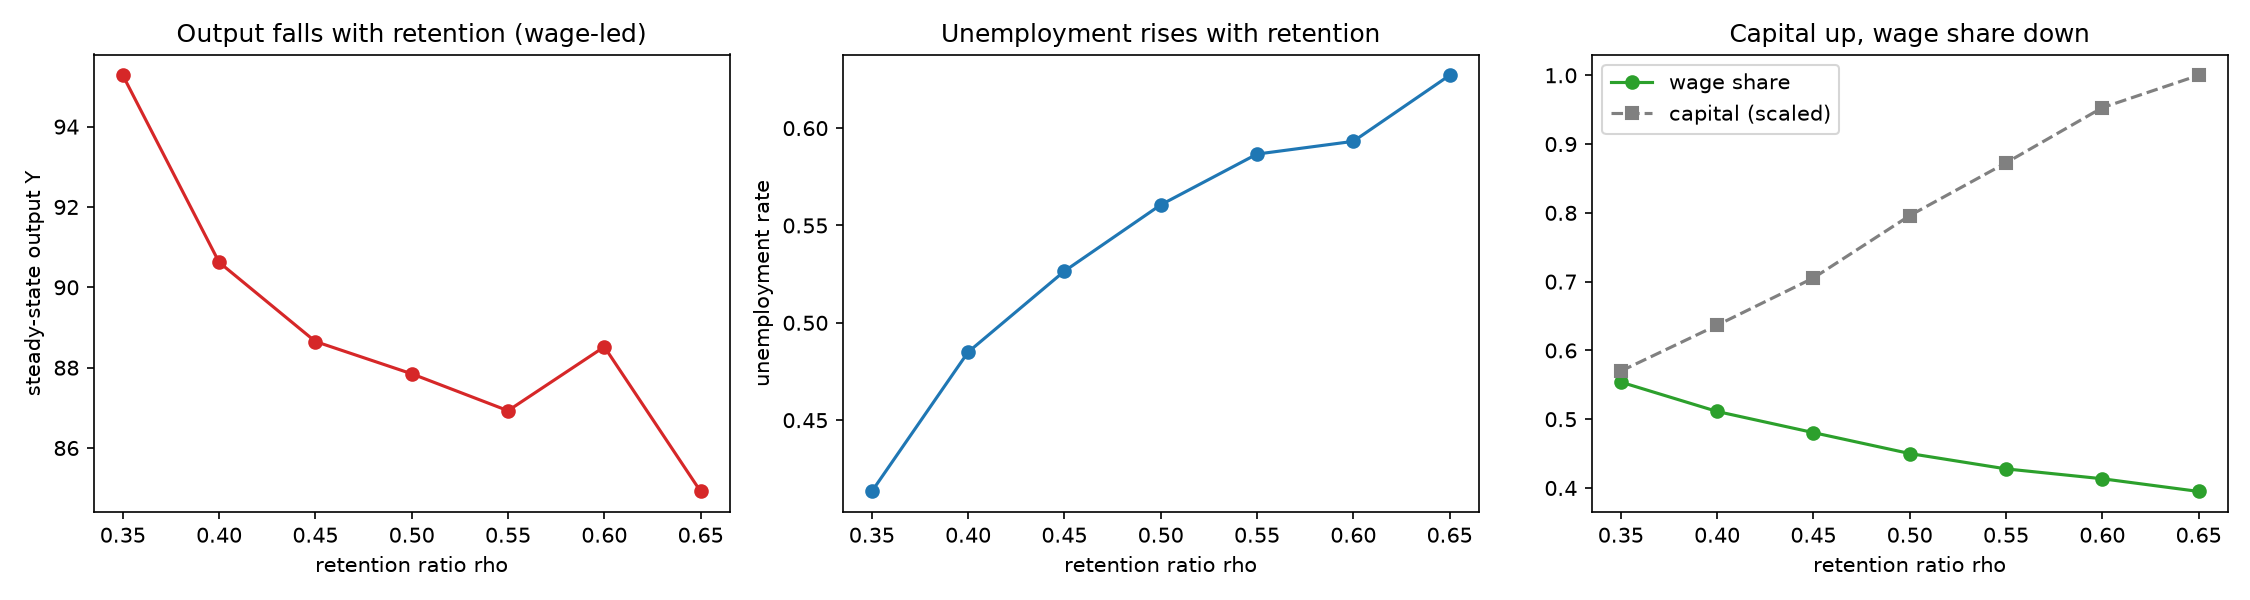
\includegraphics[width=0.82\textwidth]{retention_sweep.png}
\caption{Retention sweep at $\sigma = 1$: output falls while capital rises.
(Illustrative three-seed run; the canonical figures are those of
\cref{tab:baseline}.)}
\label{fig:retention}
\end{figure}
